\section{UI-Elemente}
\subsection{Buttons}
\begin{itemize}
	\item \textbf{Primär:} Z.B.\ „Anmelden“, „Speichern“, „Weiter“, „Abbrechen“, „Fertig“.
	\item \textbf{Sekundär:} Z.B.\ „Zurück“, „Erneut erinnern“, „Kommentar speichern“.
	\item \textbf{CTA (Call-to-Action):} Z.B.\ „Aufforderung zur Medikamenteneinnahme“.
\end{itemize}

Primäre Buttons sind Blau ausgefüllt (\texttt{\#45B3CB}). Sekundäre Buttons sind nicht ausgefüllt, besitzen jedoch einen blauen Rand (\texttt{\#45B3CB}). Dies signalisiert dem Menschen welcher Button für den weiteren Prozess am wichtigsten ist. Sekundäre Buttons zeigen an, dass hier weitere Funktion und zusätzliche Informationen verfügbar sind.

\begin{figure}[h!]
	\centering
	\begin{minipage}{0.45\linewidth}
		\centering
		\includegraphics[width=\linewidth]{images/Primärer Button}
		\caption{Primärer Button}
		\label{fig:primarer-button}
	\end{minipage}
	\hfill
	\begin{minipage}{0.45\linewidth}
		\centering
		\includegraphics[width=\linewidth]{images/Sekundärerer Button}
		\caption{Sekundärer Button}
		\label{fig:sekundarerer-button}
	\end{minipage}
\end{figure}

\subsection{Input-Felder}
\begin{itemize}
	\item Textfelder für Telefonnummern, Codes, Geburtsdaten, Symptombeschreibungen.
	\item Datepicker für Zeit und Datum.
	\item Kommentartextfelder (max. 1000 Zeichen).
\end{itemize}

\vspace{-2.5em}

\begin{figure}[h!]
	\centering
	\begin{minipage}{0.45\linewidth}
		\centering
		
\includegraphics[width=\linewidth]{images/Inputfeld}
		\label{fig:inputfeld}
	\end{minipage}
	\hfill
	\begin{minipage}{0.45\linewidth}
		\centering
		\vspace{1.5cm} % ggf. anpassen, um das rechte Bild zu senken
		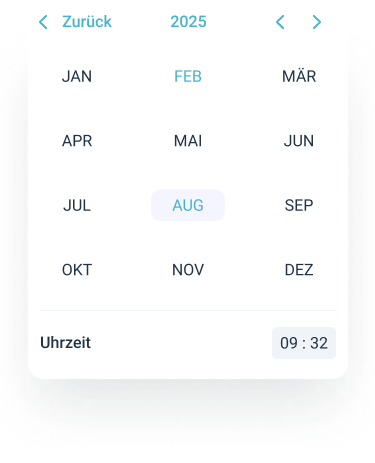
\includegraphics[width=\linewidth]{images/Geburtsdatum}
		\label{fig:geburtsdatum}
	\end{minipage}
	
	\vspace{-2.5em} % <-- negativen Wert anpassen, um Caption nach oben zu rücken
	\caption{Links: Inputfeld für Texte (z.\,B. Kommentar an den Arzt bei einer hohen Blutdruckmessung). 
		Rechts: Inputfeld für eine Datumsangabe (hier im Kontext des Datenexports).}
	\label{fig:input-und-datum}
\end{figure}



\newpage

\subsection{Dropdowns \& Listen}
\begin{itemize}
	\item Dropdowns für Datumsauswahl, Messrhythmus (z.B. täglich, wöchentlich).
	\item Listen für Kontakte, Erinnerungen, Messwerte, Medikation.
\end{itemize}

\begin{figure}[!h]
	\centering
	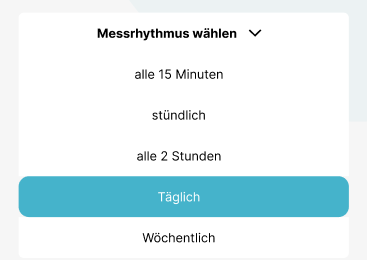
\includegraphics[width=0.45\linewidth]{images/Dropdown}
	\caption{Dropdown-Menü für den Messrhythmus bei Blutdruck \& Puls}
	\label{fig:dropdown}
\end{figure}

\subsection{Navigation}
\begin{itemize}
	\item Hauptmenü mit Modulen wie Erinnerungen, Kontakte, Blutdruck \& Puls, Datenexport, Symptomtagebuch.
	\item Onboarding-Seiten für Registrierung, Einführung, Konfiguration.
\end{itemize}

\subsection{States (Normal, Hover, Disabled, Active)}
\begin{itemize}
	\item \textbf{Normal:} Standardzustand bei Buttons, Eingabefeldern.
	\item \textbf{Disabled:} Buttons ausgegraut, wenn Eingaben fehlen oder Funktion nicht verfügbar ist.
	\item \textbf{Active:} Aktiver Menüpunkt oder laufende Messung (z.\,B.\ Fortschrittsanzeige „30\,\%“).
\end{itemize}

\begin{figure}[!h]
	\centering
	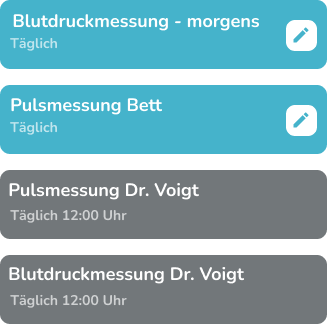
\includegraphics[width=0.4\linewidth]{images/states}
	\caption{\texttt{Normale} (Blau) und \texttt{Disabled} (Grau) States beim Screen zur Verwaltung der automatischen Messungen.}
	\label{fig:states}
\end{figure}

\newpage
